\documentclass{article}

% AlpaSim technical report (PAI track), team amanupg. Built on the organisers' template
% (alpasim_technical_report.tex, neurips_2026.sty in this folder); not a NeurIPS submission.
% DRAFT 2026-10-20. Items marked TODO need Aman's input or the official v5 result.
\PassOptionsToPackage{numbers}{natbib}
\usepackage[preprint]{neurips_2026}
\makeatletter
\renewcommand{\@noticestring}{}
\makeatother

\usepackage[utf8]{inputenc}
\usepackage[T1]{fontenc}
\usepackage{hyperref}
\usepackage{booktabs}
\usepackage{graphicx}
\usepackage{xcolor}
\usepackage{amsmath}
\usepackage{tikz}
\usetikzlibrary{positioning,arrows.meta,fit}

\newcommand{\todo}[1]{\textcolor{red}{[TODO: #1]}}

\title{Route Snap: Keeping a Zero-Shot Vision-Language-Action Driver on Its Route\\
\large AlpaSim E2E Closed Loop Challenge Technical Report (PAI track)}

\author{
  Team amanupg \\
  \todo{author name(s), organization} \\
  \texttt{\todo{contact email}}
}

\begin{document}
\maketitle

\begin{abstract}
Our PAI-track entry runs NVIDIA's Alpamayo~1.5 vision-language-action model zero-shot, without any training,
behind a thin closed-loop driver. A failure analysis of 120 local closed-loop scenes showed that most
lane-corridor exits happen where the recorded driver changed lane or took an exit and the model kept its lane,
in every one of six flow samples, so no sample selection can recover them. \emph{Route snap} detects when the
model's plan leaves the provided route waypoints by more than 2\,m on a near-straight road, and then drives a
smooth path onto the route at the model's own speed. It adds no model calls. On 120 scenes on H100 GPUs, the
evaluation hardware, it raises the local mean scene score from 0.657 to 0.728 (+0.071, 90\% bootstrap interval
[+0.011,\,+0.131]) and cuts corridor exits from 23 to 13. We also report what did not help, including a
route-following sample chooser whose gain on one GPU type vanished on the evaluation GPU type.
\end{abstract}

\section{Method summary}
The policy is the public Alpamayo~1.5 (10B) model~\cite{alpamayo15} with int8 weight-only quantization, served by
our gRPC \texttt{egodriver} implementation. It replans at 1\,Hz from the four front-facing cameras and the ego
history, and between replans it serves the last plan re-anchored to the current pose. A post-processing step,
\emph{route snap}, compares each new plan with the route waypoints the simulator provides. When the plan leaves the
route on a near-straight road, it replaces the plan's geometry with a path onto the route and keeps the plan's speed
profile (Fig.~\ref{fig:system}).

\begin{figure}[h]
\centering
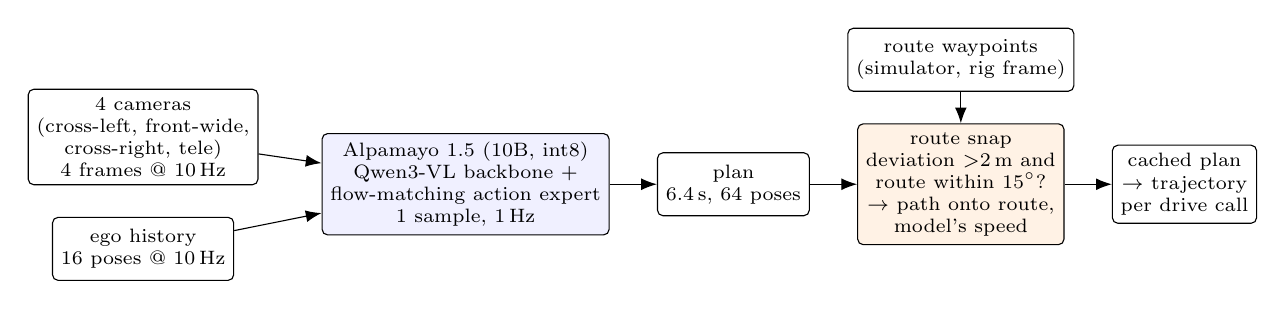
\begin{tikzpicture}[node distance=4mm and 6mm, font=\scriptsize,
  box/.style={draw, rounded corners=2pt, align=center, minimum height=8mm, inner sep=3pt},
  ar/.style={-{Latex[length=2mm]}}]
\node[box] (cam) {4 cameras\\(cross-left, front-wide,\\cross-right, tele)\\4 frames @ 10\,Hz};
\node[box, below=of cam] (ego) {ego history\\16 poses @ 10\,Hz};
\node[box, right=8mm of cam, yshift=-6mm, fill=blue!6] (a15) {Alpamayo 1.5 (10B, int8)\\Qwen3-VL backbone +\\flow-matching action expert\\1 sample, 1\,Hz};
\node[box, right=of a15] (plan) {plan\\6.4\,s, 64 poses};
\node[box, right=of plan, fill=orange!10] (snap) {route snap\\deviation $>$2\,m and\\route within 15$^\circ$?\\$\rightarrow$ path onto route,\\model's speed};
\node[box, above=of snap] (route) {route waypoints\\(simulator, rig frame)};
\node[box, right=of snap] (out) {cached plan\\$\rightarrow$ trajectory\\per drive call};
\draw[ar] (cam) -- (a15); \draw[ar] (ego) -- (a15); \draw[ar] (a15) -- (plan); \draw[ar] (plan) -- (snap);
\draw[ar] (route) -- (snap); \draw[ar] (snap) -- (out);
\end{tikzpicture}
\caption{System. Only route snap (orange) is new relative to running Alpamayo~1.5 as released.}
\label{fig:system}
\end{figure}

\section{Policy description}
\textbf{Observations.} The front-wide, cross-left, cross-right and front-tele cameras are the four Alpamayo was
trained with. Each provides the last four frames at 0.1\,s spacing, resized to $576\times320$. The ego history is
16 poses at 0.1\,s in the current rig frame. We use no reasoning text and no navigation text: route text in the
prompt gave no gain (+0.002).

\textbf{Model output.} The flow-matching action expert outputs 64 poses at 0.1\,s ($x$, $y$, heading) in the rig
frame. We draw one sample per replan; the submitted v0.3 used the same configuration.

\textbf{Route snap.} The simulator sends route waypoints, the recorded path about 40--80\,m ahead, in the rig frame.
For a plan $P$ we compute the deviation $d$, the mean distance from the route waypoints within the plan's reach to the
polyline of $P$. Measuring from the route side avoids penalising long plans at highway speed. A snap fires when:
(i) $d > 2$\,m, or $d > 1$\,m while a snap is already under way (hysteresis, so a lane change is not abandoned
halfway); and (ii) both the direction to the first waypoint and the route's direction there lie within $15^\circ$ of
the car's heading. The snapped geometry is a cubic Hermite curve from the car (current heading) to the first
waypoint, arriving along the route direction, followed by the route. It is re-timed with the model's plan: pose $k$
lies on the new path at the arc length the original plan covered by step $k$, so the model keeps control of speed.
The angle guard matters. Without it, snapping on turns cut corners: the curve to a waypoint about 40\,m ahead ignores
the road's real geometry, which cost $-$0.042 on one 40-scene batch through offroad and low-progress outcomes. With
the guard, route snap acts on lane changes and exits, the cases where all samples kept their lane.

\section{Resources and training}
\textbf{No training and no private resources.} All weights are used as released. \textbf{Pretrained weights:}
Alpamayo~1.5~10B~\cite{alpamayo15} (NVIDIA; weights under OpenMDW-1.1, code under Apache-2.0), including its
Qwen3-VL-8B backbone, and the Qwen3-VL-2B-Instruct processor configuration~\cite{qwen3vl} (Apache-2.0).
\textbf{Code:} our driver's gRPC structure follows NVIDIA's VAVAM sample driver (Apache-2.0); the multi-camera
input, the plan cache and route snap are ours. \textbf{Data:} no training data. For local closed-loop evaluation
only, we used the AlpaSim simulator~\cite{alpasim} and 120 scenes of the PAI-AV NuRec curated validation suite
under its access terms. Route snap uses only the route waypoints that the simulator sends to every driver; it never
uses the recorded ground-truth trajectory. \todo{confirm wording of the PAI-AV private-resource statement (none
used).}

\section{Runtime and reproducibility}
\textbf{Inference.} Weights load in bf16 and are quantized with torchao int8 weight-only. The token-embedding table
stays on the CPU, and all GPU work runs on one worker thread. That thread is required for the memory budget: with
predict calls on several gRPC threads, driver memory on H100 grew from 14.6 to 17.3\,GiB. Measured with
\texttt{nvidia-smi}, the driver process uses 14.2--14.6\,GiB, under the 16\,GiB limit. One replan takes 0.96\,s on an
L40S with a single session and 1.5--1.9\,s on H100 with four concurrent sessions. Route snap is a few milliseconds of
NumPy. The submitted v0.3, with the same model call, finished the official PAI run in 9{,}474 of 14{,}400\,s.

\textbf{Local evaluation protocol.} We used 120 curated-validation PAI scenes, compared per scene between
configurations, with 90\% bootstrap intervals. Two findings shaped every decision. (1) \emph{Reruns of the same
configuration on the same GPU type are nearly deterministic}: two Blackwell runs gave 0.692 and 0.692, and batch
means agreed within 0.006. (2) \emph{GPU type changes results}. The same configuration scored 0.031 lower on H100
than on RTX PRO 6000 (Blackwell), and a route-following best-of-6 sample chooser that gained +0.054 on Blackwell
gained only +0.005 on H100. We therefore made the final choice on H100, the evaluation GPU. Our local H100 score for
v0.3 (0.657) is 0.046 above its official score (0.611).

\begin{table}[h]
\centering\small
\begin{tabular}{lccc}
\toprule
Configuration (H100, 120 scenes) & mean scene score & vs v0.3 [90\%] & corridor exits / passes \\
\midrule
v0.3 (submitted: Alpamayo 1.5, 1 sample, 1\,Hz) & 0.657 & -- & 23 / 67 \\
+ best-of-6 route chooser & 0.662 & +0.005 [$-$0.044, +0.054] & -- \\
+ chooser + route snap & 0.715 & +0.058 [$-$0.003, +0.122] & 13 / 75 \\
\textbf{+ route snap (final, v5)} & \textbf{0.728} & \textbf{+0.071 [+0.011, +0.131]} & 13 / 75 \\
\bottomrule
\end{tabular}
\caption{Local closed-loop results. Official results: v0.3, PCS 2143 (scene score 0.611, at-fault distance 0.795);
v5, \todo{official result}.}
\label{tab:main}
\end{table}

\textbf{What did not help.} Each item is measured on 120 scenes against the configuration it modified:
\begin{itemize}
\item all six cameras: $-$0.023;
\item a hybrid using the rear cameras for speed only: $-$0.052;
\item replanning at 2\,Hz: $-$0.045;
\item driving the planned path 15\% faster: $-$0.307;
\item lower sampling temperature: 0.000;
\item 12 samples instead of 6: no gain, at +15\% time;
\item pulling the far part of the plan onto the route: $-$0.002;
\item a waypoint memory that lets snap follow turns: +0.003, then $-$0.078 on one batch.
\end{itemize}

\section{Limitations and safety considerations}
\textbf{Rear-end collisions from following too slowly.} Most remaining low-progress outcomes are rear-end hits by
replayed traffic: our car drives slower than the recorded car behind it, which is not reactive. These count as not at
fault but end the scene early. Every speed-increasing change we tried added at-fault collisions.

\textbf{Missed turns.} Route snap is disabled on turns, so a model that goes straight where the route turns still
leaves the corridor. Remembering earlier route waypoints recovers the turn geometry, and it fixed several such scenes,
but driving the recorded curve at the model's speed broke others.

\textbf{Route snap trusts the route.} When the route stays in our lane and the model swerves, for example around an
obstacle, a snap can override the swerve. We saw one such case (a corridor exit). Snap keeps the model's speed
profile, but it does not re-check the new path for obstacles. A deployed system would need an explicit
collision check on the snapped path.

\textbf{Evaluation.} Local scores are about 0.05 above official ones, and 40-scene batch results vary by up to
$\pm$0.1 between configurations, so single-batch gains are not reliable. On our cluster, H100 runs saw intermittent
CUDA launch failures in the driver process (6 of 25 batches). We detected them, discarded those batches and reran
them. They did not occur on Blackwell, and we attribute them to the local driver stack.

\section*{References}
\begin{thebibliography}{9}
\bibitem{alpamayo15} NVIDIA. \newblock Alpamayo 1.5. \newblock \url{https://huggingface.co/nvidia/Alpamayo-1.5-10B}, 2026.
\bibitem{qwen3vl} Qwen Team. \newblock Qwen3-VL. \newblock \url{https://huggingface.co/Qwen/Qwen3-VL-8B-Instruct}, 2025.
\bibitem{alpasim} NVIDIA. \newblock AlpaSim. \newblock \url{https://github.com/NVlabs/alpasim}, 2026.
\end{thebibliography}

\end{document}
